\section{Overview}
The gem5 Simulator \cite{binkert_gem5_2011} is a state-of-the-art hardware 
simulator used not only for architecture research, but also by the companies 
which develop the hardware it simulates. ARM, for example, have detailed their 
use of it at the ARM research summit in 2017. It is the result of merging two 
simulators in 2011: the m5 simulator, which had great support for multiple 
hardware architectures and ISAs, and the GEMS simulator, whose main focus was 
memory simulation and hence allowed for detailed memory models and various 
cache coherence protocols \cite{binkert_gem5_2011}.

Due to the enormous complexity of such a piece of software, the way to start 
using gem5 is to download and build from source \cite{noauthor_gem5_nodate-2}. 
Building the simulator can be a bit complicated, due to it being sensitive to 
various system tools and configurations. The gem5 Simulator uses \texttt{scons} 
as its build tool. Specifically, it seems to rely on the Python 2 version of 
\texttt{scons} (and also uses Python 2 for its other Python scripts) despite 
Python 2 having been officially deprecated on the 1\textsuperscript{st} of 
January 2020, with the move to do so being announced well in advance 
\cite{noauthor_sunsetting_nodate}. However, this can be easily fixed by using a 
Python 2 virtual environment. The specific version of the GNU Compiler 
Collection (GCC) also seems to affect things. I was using GCC version 9.3.0 
which must have more warnings than the version used by the gem5 developers, as 
it failed to build gem5 due to the \texttt{-Werror} flag being turned on. This 
flags turns compiler warnings, which normally highlight suspicious areas of 
code but still lets the build go ahead, into errors which do not let the build 
go ahead. The user can tell the compiler that some warnings are exceptions to 
the \texttt{-Werror} flag, but due to the number of warnings I was getting, it 
was simpler to remove the flag from the \texttt{scons} configuration found in 
the \texttt{SConstruct} file. There are also a number of packages that the 
build script might recommend one installs, most notably the Google Performance 
Tools (gperftools) \cite{noauthor_google_nodate} which they suggest improves 
performance by 12\%. Once the necessary software, packages, etc. have been 
installed and configured, the build process takes around 20-30 minutes when 
building using 13 threads on an 8\textsuperscript{th} generation Intel Core i7 
processor, which also says something about the scale and complexity of gem5.

\section{Configuration and Setup}
    \subsection{The gem5 binary}
    There are two parts of gem5 that can be configured: the simulator binary 
    and its configuration files. The binary produced by \texttt{scons} supports 
    a number of flags which allow the user to specify things like the output 
    directory, whether to redirect gem5's standard output and/or standard error 
    streams, and what to call the various files being output. There are also 
    anumber of debug flags for developing gem5 itself. The most important of 
    the flags is arguably the \texttt{--outdir} flag used for specifying the 
    output directory. When running multiple simulations side by side, if no 
    directory is specified, i.e. the default \texttt{m5out} directory is used, 
    each instance will try to write to the same files as the others, resulting 
    in non-deterministic race conditions in terms of which process was the last 
    to write to the file, leading to unusable, interweaved output.

    \subsection{Python configuration scripts}
    After the flags, gem5 takes a Python script containing the setup(s) to run. 
    Since this is a regular Python script, it is possible to add command line 
    arguments here as well, allowing for control over the system configuration 
    without having to change the Python file itself. The gem5 Simulator comes 
    with a number of example scripts for ARM system simulation, located in the 
    \texttt{gem5/configs/example/arm} directory. The scripts provide examples 
    for syscall emulation, full system simulation, and full system simulation 
    with power models. Syscall emulation is faster than full system simulation 
    because it only simulates the system calls and their results, and not the 
    disks, memory, kernel, operating system, etc. Because of this, it is also 
    less precise. Full system simulation takes a while and requires a lot more 
    setup. The system has to be specified in its entirety: The full system (FS) 
    section of the ``Learning gem5'' book \cite{lowe-power_full_nodate} shows 
    how in order to run a full system simulation, the various caches, disks, 
    memory controllers, and North and South Bridges (for x86 system simulation) 
    have to be specified as Python objects. Fortunately, the 
    \texttt{devices.py} file in the example scripts directory already has all 
    of this implemented for ARM full system simulation. The example power model 
    script contains some very simple power models and is likely mainly to show 
    how the power models are specified and added to the objects that support 
    them. By default, the full system scripts support flags allowing to specify 
    the frequency and number of big and LITTLE cores; where the kernel, disk, 
    bootloader, and bootscript are located; whether to instantiate and simulate 
    caches; what CPU type to use; whether to restore from a checkpoint; and 
    much more.
    
    \subsection{Bootscripts, systems, and m5 instructions}
    One of the arguments that must be passed to the simulated system (either 
    hardcoded in the Python configuration script or passed via a flag) is the 
    path to the bootscript to run once the OS has booted. The gem5 Simulator 
    comes with a couple of bootscripts, but these are for simulating distributed
    compute nodes, e.g. a compute cluster with multiple physical systems 
    collaborating and communicating over a network, and therefore contains a 
    lot of networking and other things that are unnecessary for this project. 
    However, it does provide some insight into how to write these. As far as I 
    can tell, even though the bootscripts all end in \texttt{.rcS}, the script 
    itself is simply a bash script with most of the usual bash builtins 
    supported. One slight complication is that the \texttt{PATH} environment 
    variable seems to always be unset so absolute paths to programs must be 
    specified rather than assuming they are available, e.g. you have to use 
    \texttt{/bin/ls} to list directory contents because \texttt{ls} is not on 
    the \texttt{PATH}.
    
    In order to simulate a full system, a kernel, disk, and bootloader must be
    provided. The gem5 website hosts a number of Linux disk images at
    \cite{noauthor_index_2020}. However, the gem5 website has recently been 
    modernised and in the process the file which displayed an index of 
    \cite{noauthor_index_2020} seems to have disappeared. Therefore the way to 
    get these system images is to use an old version of the m5 Simulator's 
    webpage \cite{noauthor_index_2017} which \textit{does} have an index, copy 
    the name of the file, and append it to the URL of 
    \cite{noauthor_index_2020}. This downloads the most recent version of the 
    system image from the official gem5 website rather than relying on the old 
    website(s) still being maintained. The system downloaded will typically 
    contain \texttt{disk} and \texttt{binaries} subdirectories. The 
    \texttt{disk} directory should contain a disk image (\texttt{.img}) file 
    with BusyBox \cite{noauthor_busybox_nodate} and an \texttt{init} process 
    pre-configured. It is possible to mount the disk image through a loopback 
    device on Linux, using the command
    \begin{lstlisting}
    sudo mount -o loop,offset=32256 \
        /path/to/disk-image.img /path/to/mountpoint
    \end{lstlisting}
    The \texttt{offset} specifies where the file system starts on the disk 
    image and is derived from 63 sectors $\times$ a 512-byte sector size. 
    Mounting the disk image can be useful in order to find or double-check the 
    absolute paths of certain programs for use in a bootscript, or to place 
    custom programs there in order to be able to run them in the simulator. The 
    \texttt{m5} program, which is specific to interfacing with the simulator 
    from within the simulated system, comes ``pre-installed'' on the 
    gem5-provided disk images.
    
    The \texttt{m5} program is typically located at \texttt{/sbin/m5} and is 
    used to pass instructions to the simulator from within the simulated system.
    If the program is run without passing any arguments, it will print a list of
    the supported commands. The most useful one is \texttt{m5 checkpoint} which
    creates a checkpoint at the current simulation tick.
    
    \subsection{CPU types and checkpointing}
    By default, gem5 provides 3 CPU types for ARM system simulation: `timing',
    `atomic', and `exynos'. The last one likely refers to the Samsung Exynos 
    platform which may have special simulation requirements beyond the default 
    ARM systems. As we were not using this platform, I did not look further 
    into this setting. The `timing' and `atomic' CPU types have a key 
    difference: the atomic CPU type is a simplified CPU where every instruction 
    is atomic, i.e. it happens in one go and does not incur latency. This 
    results in much faster simulations (around 20 minutes to boot Linux 
    compared to around $1\frac{1}{2}$-2 hours using the timing CPU) at the cost 
    of 
    simulation realism. In reality, CPU instructions have a latency associated 
    with them, and so some instructions take longer than others. The timing CPU 
    models these latencies. As a result, it is a much more realistic simulation,
    at the cost of taking a lot longer to simulate.
    
    The atomic CPU type is extremely useful for ``fast-forwarding'' and 
    ``checkpointing''. As previously mentioned, running a full system 
    simulation with the timing CPU takes a long time to even get the operating 
    system booted. This is impractical if all we are interested in is the 
    program being run once the operating system has booted, e.g. if we are 
    running a benchmark, as only using the timing CPU would result in long wait 
    times due to a process that the researcher is not interested in. To mitigate
    this, gem5 allows the user to create and resume from checkpoints: stores of 
    exact system layout at a specific point in time, which can be used to resume
    the simulation from this state without needing to redo all the simulation 
    preceding it. When resuming from a checkpoint, the CPU type can be changed.
    This allows us to ``fast-forward'' parts of the system we are not interested
    in by using the atomic CPU and calling the \texttt{m5 checkpoint} 
    instruction from within the bootscript, before the line(s) where the 
    bootscript starts the benchmark.
    \begin{lstlisting}[language=bash, caption=Example bootscript using 
    checkpointing, basicstyle=\sffamily\footnotesize]
    #!/bin/bash
    
    echo "bootscript.rcS is running"
    
    /sbin/m5 checkpoint
    echo "Starting workload"
    /path/to/workload
    
    echo "Workload done, exiting simulation."
    /sbin/m5 exit
    \end{lstlisting}
    Once the bootscript has created the checkpoint, we can then interrupt the 
    simulation and restart it with the timing CPU using the \texttt{--cpu-type} 
    flag, and specify the path to the checkpoint to restore from using the 
    \texttt{--resume-from} flag. Unfortunately, it seems that the bootscript is 
    loaded into memory and hence stored along with the checkpoint, meaning 
    separate bootscripts have to be created and fast-forwarded for separate 
    workloads. Swapping the bootscript when resuming does not seem to have any 
    effect and the simulator will instead use the bootscript that was initially 
    passed to the simulator when fast-forwarding.
    
\section{Customising the setups}
While the provided Python scripts help define almost everything, there are 
certain things that can be modelled which are not present in the scripts, due to
their already high complexity. In order to include these things in the 
simulation, it is therefore necessary to extend and/or modify the provided 
scripts.

    \subsection{Voltage and Frequency Domains}
    Part of this project was to look at whether scheduling and DVFS can be 
    combined to achieve more intelligent, power efficient schedules. Therefore, 
    we need the system we are simulating to have DVFS capabilities. In gem5, 
    adding DVFS to a simulation is done by assigning ``Frequency Domains'' to 
    certain objects. Since DVFS impacts the frequency, i.e. the clock speed, of 
    the object, any \texttt{ClockedObject} (which the CPU implementations are a 
    subclass of) can be assigned a Clock Domain. The documentation for adding 
    DVFS to a system is only available on the old website 
    \cite{noauthor_experimenting_2019} and it does not detail how to add DVFS 
    for the \texttt{fs\_bigLITTLE.py} configuration. In order to figure this 
    out, it is required to look at the script \textit{and} some of the gem5
    source code.
    \begin{lstlisting}[caption=Lines 42-52 from 
    \texttt{gem5/src/sim/VoltageDomain.py}, basicstyle=\sffamily\footnotesize,
    language=Python]
class VoltageDomain(SimObject):
    type = 'VoltageDomain'
    cxx_header = "sim/voltage_domain.hh"
    
    # Single or list of voltages for the voltage domain. If only a single
    # voltage is specified, it is used for all different frequencies.
    # Otherwise, the number of specified voltges and frequencies in the clock
    # domain (src/sim/ClockDomain.py) must match.  Voltages must be specified in
    # descending order. We use a default voltage of 1V to avoid forcing users to
    # set it even if they are not interested in using the functionality
    voltage = VectorParam.Voltage('1V', "Operational voltage(s)")
    \end{lstlisting}
    \begin{lstlisting}[caption=Lines 44-69 from 
    \texttt{gem5/src/sim/ClockDomain.py}, basicstyle=\sffamily\footnotesize,
    language=Python]
# Abstract clock domain
class ClockDomain(SimObject):
    type = 'ClockDomain'
    cxx_header = "sim/clock_domain.hh"
    abstract = True

# Source clock domain with an actual clock, and a list of voltage and frequency
# op points
class SrcClockDomain(ClockDomain):
    type = 'SrcClockDomain'
    cxx_header = "sim/clock_domain.hh"
    
    # Single clock frequency value, or list of frequencies for DVFS
    # Frequencies must be ordered in descending order
    # Note: Matching voltages should be defined in the voltage domain
    clock = VectorParam.Clock("Clock period")
    
    # A source clock must be associated with a voltage domain
    voltage_domain = Param.VoltageDomain("Voltage domain")
    
    # Domain ID is an identifier for the DVFS domain as understood by the
    # necessary control logic (either software or hardware). For example, in
    # case of software control via cpufreq framework the IDs should correspond
    # to the neccessary identifier in the device tree blob which is interpretted
    # by the device driver to communicate to the domain controller in hardware.
    domain_id = Param.Int32(-1, "domain id")
    \end{lstlisting}
    By examining the source code of the Voltage and Clock Domain objects, we 
    discover several things not apparent in the guide/documentation:
    \begin{enumerate}
        \item Voltage and frequency points have to be specified in sorted,
              descending order.
        \item There can either be one voltage value for all frequency steps or
              there must be exactly the same number of voltage and frequency 
              steps.
        \item Clock domains have an ID which must be unique.
    \end{enumerate}

    When looking at the provided system devices in 
    \texttt{gem5/configs/example/arm/devices.py}, the \texttt{CpuCluster} 
    constructor already has constructor support for specifying voltage and 
    clock domains.
    \begin{lstlisting}[caption=The \texttt{CpuCluster} constructor, 
    language=Python, basicstyle=\sffamily\footnotesize]
class CpuCluster(SubSystem):
    def __init__(self, system,  num_cpus, cpu_clock, cpu_voltage,
                 cpu_type, l1i_type, l1d_type, wcache_type, l2_type):
    \end{lstlisting}
    Passing a list of values to the \texttt{cpu\_clock} and 
    \texttt{cpu\_voltage} arguments constructs the relevant objects inside the 
    \texttt{CpuCluster} object. The only part that needs changing is that the 
    clock domains are not given an ID. This causes the simulator to crash, as 
    the logic detects that the default ID of $-1$ was given and errors with a 
    message explaining that clock domains must have a unique ID. As part of the 
    project, an Odroid N2 board was acquired. By examining its DVFS capabilities
    using the \texttt{cpupower} tool, it seems the most common setup is to have
    one DVFS domain per cluster, i.e. per big and LITTLE `part' of the setup.
    Therefore, I change the line initialising the voltage domain to assign an ID
    based on the number of clusters in the system. This will return 0 for the 
    first cluster, i.e. cluster 0, and 1 for the second cluster.
    \begin{lstlisting}[caption=Modified line 126 of \texttt{devices.py}, 
    language=Python, basicstyle=\sffamily\footnotesize]
    self.clk_domain = SrcClockDomain(clock=cpu_clock,
                                     voltage_domain=self.voltage_domain,
                                     domain_id=system.numCpuClusters())
    \end{lstlisting}
    
    With the devices modified to correctly set up the DVFS objects in the 
    simulator, the only thing that remains to be changed is the 
    \texttt{fs\_bigLITTLE.py} file. In an attempt to model DVFS as realistically
    as possible, I used clock and voltage steps from the Odroid N2 board that I 
    had on hand. The clock steps were collected through the \texttt{cpupower} 
    tool. The voltage steps were harder figure out where to find. It turns out 
    that Linux provides some insight into the voltage values through the sysfs, 
    i.e. the \texttt{/sys} file system. There are a number of voltage 
    regulators at \texttt{/sys/class/regulator/regulator.\{0,1,2\}}. By using 
    the \texttt{userspace} frequency governor, which scales the frequency to 
    whatever the user specifies, and the \texttt{cpupower} tool to adjust the 
    frequency, I was able to narrow down that regulators 1 and 2 control the 
    voltage of the LITTLE and big clusters respectively. Regulator 0 seems to 
    not do anything, as running \texttt{cat} on the \texttt{regulator.0/name} 
    outputs the value ``\texttt{regulator-dummy}'', indicating that the 
    regulator is unlikely to control anything.
    \begin{figure}[H]
        \centering
        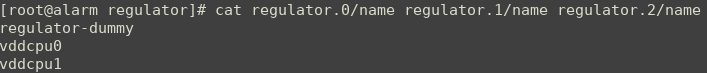
\includegraphics[width=0.9\linewidth]{../screenshots/odroid-stuff/regulator-names.png}
        \caption{The names of the regulators on the Odroid N2 board}
    \end{figure}

    \texttt{CpuCluster}    \todo{show+explain extending CpuCluster}
    
    \subsection{Power Models}
    
    \subsection{Output resolution}



\begin{itemize}
    \item explain the layouts of the various python scripts, the need to
          customise them, and what changes were made (provide code examples!)
    \item as part of the above, explain the various features that are needed for
          this dissertation and why
    \item mention the gemstone-applypower project and why its power equations
          are meant to be good
\end{itemize}